\documentclass[8pt]{extarticle}
\title{Econ 250 HW 3}
\author{Avinash Iyer}
\date{September 21, 2022}

%font setup
%
%\usepackage[math]{anttor}

%paper setup
\usepackage{geometry}
\geometry{letterpaper, portrait, margin=1in}
\usepackage{fancyhdr}

%symbols
\usepackage{amsmath}
\usepackage{amssymb}
\usepackage{hyperref}
\usepackage{gensymb}

\usepackage[T1]{fontenc}
\usepackage[utf8]{inputenc}

%chemistry stuff
\usepackage[version=4]{mhchem}
\usepackage{chemfig}

%plotting
\usepackage{pgfplots}
\usepackage{tikz}

%\usepackage{natbib}

%graphics stuff
\usepackage{graphicx}
\graphicspath{ {./images/} }

%a useful command
\newcommand{\plain}[1]{\textrm{#1}}

%code stuff
%when using minted, make sure to add the -shell-escape flag
%you can use lstlisting if you don't want to use minted
%\usepackage{minted}
%\usemintedstyle{pastie}
%\newminted[javacode]{java}{frame=lines,framesep=2mm,linenos=true,fontsize=\footnotesize,tabsize=3,autogobble,}
%\newminted[cppcode]{cpp}{frame=lines,framesep=2mm,linenos=true,fontsize=\footnotesize,tabsize=3,autogobble,}

\usepackage{listings}
\usepackage{color}
\definecolor{dkgreen}{rgb}{0,0.6,0}
\definecolor{gray}{rgb}{0.5,0.5,0.5}
\definecolor{mauve}{rgb}{0.58,0,0.82}

\lstset{frame=tb,
	language=Java,
	aboveskip=3mm,
	belowskip=3mm,
	showstringspaces=false,
	columns=flexible,
	basicstyle={\small\ttfamily},
	numbers=none,
	numberstyle=\tiny\color{gray},
	keywordstyle=\color{blue},
	commentstyle=\color{dkgreen},
	stringstyle=\color{mauve},
	breaklines=true,
	breakatwhitespace=true,
	tabsize=3
}
\usepackage{multirow}
\pagestyle{fancy}
\fancyhf{}
\rhead{Avinash Iyer}
\lhead{Econ 250 HW 3}
\begin{document}{
\renewcommand{\arraystretch}{2}
\maketitle
\section{Marginal Utility}
\subsection*{Part A}
\begin{center}
	\begin{tabular}{|c|c|c|c|c|c|c|c|c|}
		\hline
		\multicolumn{3}{|c|}{Abe} & \multicolumn{3}{|c|}{Barbara} & \multicolumn{3}{|c|}{Chuck}\\
		\hline
		$U(X)$ & $X$ & $MU_X$ & $U(X)$ & $X$ & $MU_X$ & $U(X)$ & $X$ & $MU_X$ \\
		\hline
		10 & 2 & N/A & 10 & 2 & N/A & 10 & 2 & N/A \\
		\hline
		14 & 3 & 4 & 10 & 3 & 0 & 12 & 3 & 2 \\
		\hline
		16 & 4 & 2 & 10 & 4 & 0 & 15 & 4 & 3\\
		\hline
		17 & 5 & 1 & 9 & 5 & -1 & 19 & 5 & 4\\
		\hline
		17.5 & 6 & 0.5 & 8 & 6 & -1 & 24 & 6 & 5\\
		\hline
	\end{tabular}
\end{center}
\subsection*{Part B}
Barbara is violating the ``more is better'' of preferences because increasing $X$ from 4 to 5 or 5 to 6 reduces her utility. The other two consumers, Abe and Chuck, do not violate any assumptions of preferences.
\subsection*{Part C}
It is possible that Abe and Chuck have the exact same preferences because both of their utility functions are increasing, but the units of utility are arbitrary so they might have similar preferences in real life.
\section{Preference Comparisons}
\begin{center}
	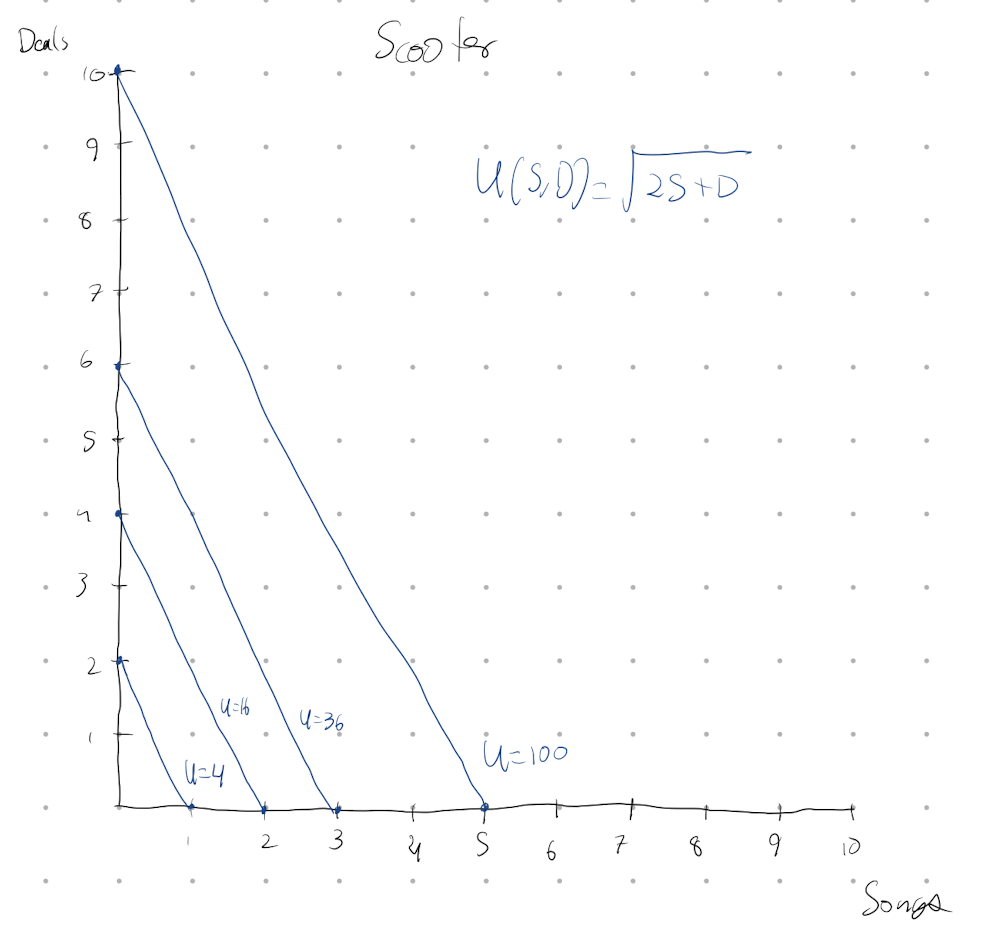
\includegraphics[width=10cm]{HW3Q2}
\end{center}
Justin and Scooter have different preferences — though songs and deals are perfect substitutes for both of them, Scooter has a stronger preference for songs (as his indifference curves are steeper) while Justin has a stronger preference for deals (as his indifference curves are shallower).
\section{Marginal rates of substitution}
\subsection*{Part A}
\subsubsection*{Subpart I}
\begin{center}
	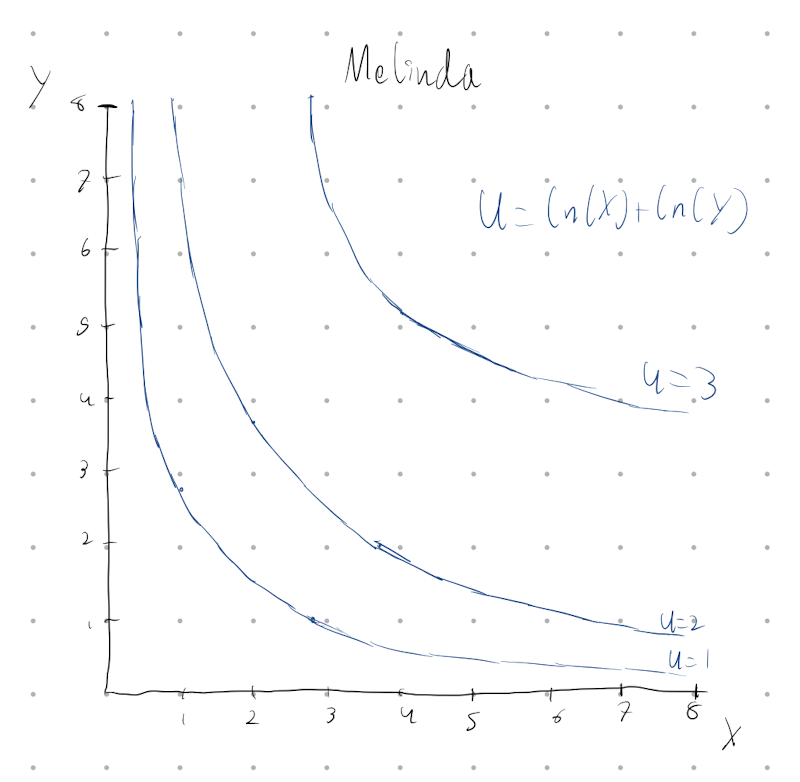
\includegraphics[width=10cm]{HW3Q3A}
\end{center}
\subsubsection*{Subpart II}
\begin{align*}
	MRS_{XY} &= \frac{MU_X}{MU_Y}\\
	&= \frac{\frac{\partial U}{\partial X}}{\frac{\partial U}{\partial Y}}\\
	&= \frac{\frac{1}{X}}{\frac{1}{Y}}\\
	&= \boxed{\frac{Y}{X}}
\end{align*}
The marginal rate of substitution means that if her preferences for an additional unit of $X$ only increases by a factor of $Y/X$, meaning that at a high number of $X$ goods, she only needs to substitute a small amount of $Y$ to retain the same utility.
\subsection*{Part B}
\subsubsection*{Subpart I}
\begin{center}
	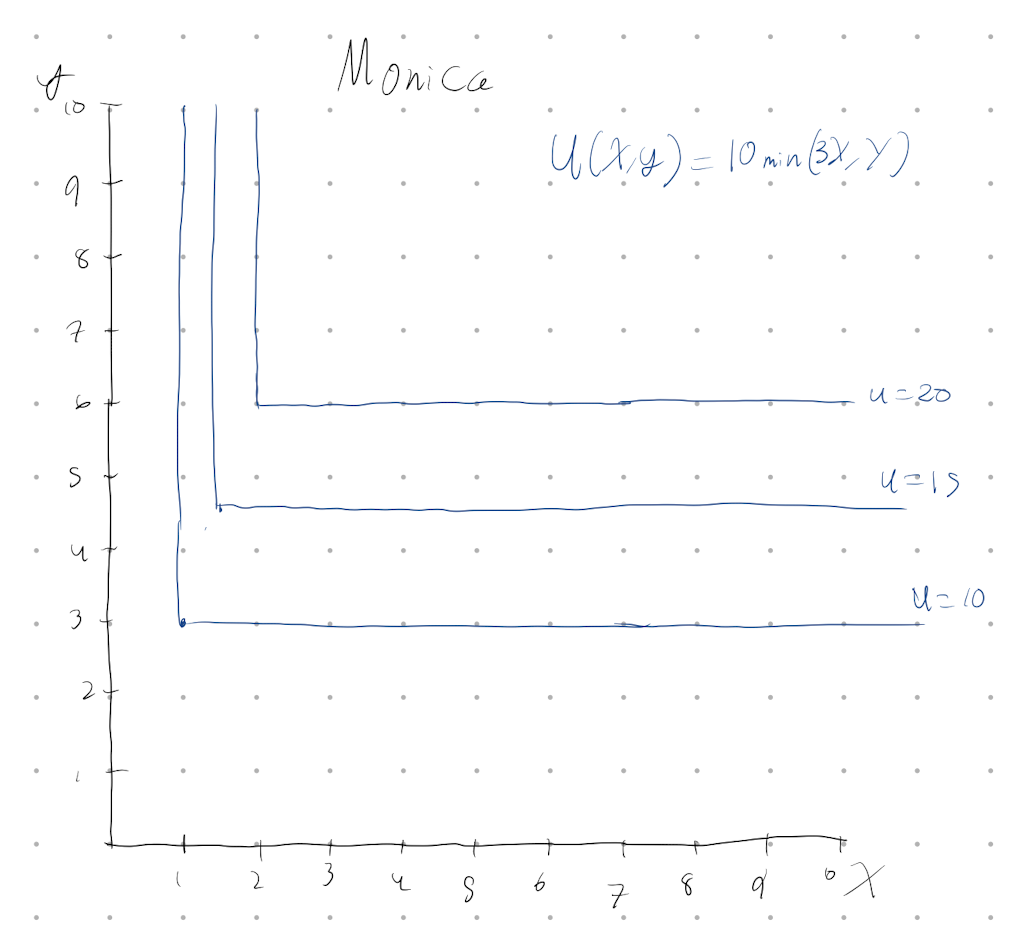
\includegraphics[width=10cm]{HW3Q3B}
\end{center}
\subsubsection*{Subpart II}
Since $3(5) > (3)$, the section of the map that contains $(5,3)$ is equivalent to the function $f(x) = 3$, so the marginal rate of substitution is equivalent to $0$, meaning that, to Monica, good $X$ and good $Y$ are perfect complements, meaning that any extra amount of good $X$ doesn't change Monica's utility at this point.
\section{Preference Violations}
\subsection*{Part A}
Mary's preferences do not satisfy the assumption of balance, as part of the indifference curve slopes upward.
\subsection*{Part B}
Edith's preferences do not satisfy the assumptions of transitivity and non-satiation as $U_2$ crosses $ U_1 $.
\section{Trades with Utility}
\begin{center}
	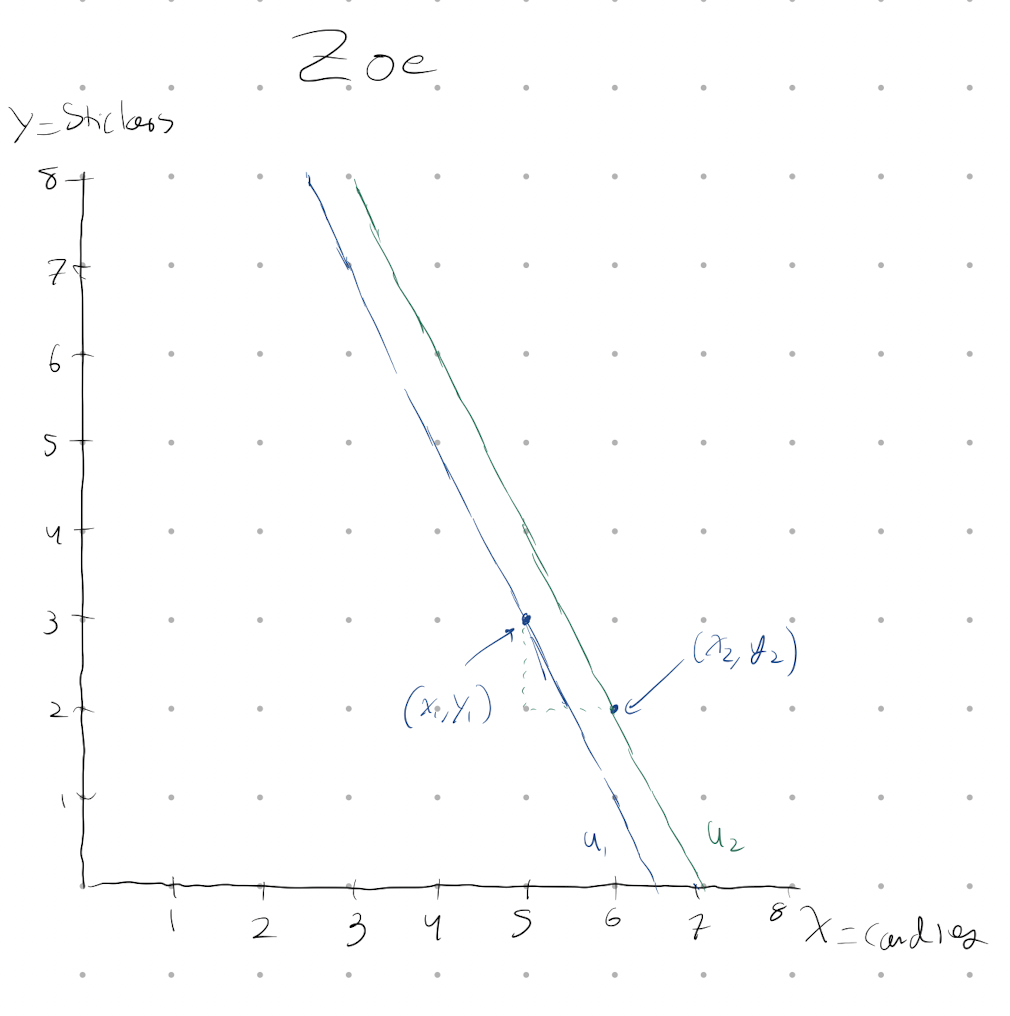
\includegraphics[width=10cm]{HW3Q5}
\end{center}
\noindent Since $ U_2 $ has a higher utility than $ U_1 $, Zoe should take the trade.
\section{Budget Constraints}
\subsection*{Part A}
\[ 10M + 5C = 150 \]
\subsection*{Part B}
The movie theater prices movies at $5$ and popcorn at $7.5$.
\subsection*{Part C}
\begin{center}
	\begin{tabular}{c|c}
		Popcorn (\$5) &	Movies (\$10), 5 movies free \\
		\hline
		0 & 20 \\
		5 & 17.5 \\
		10 & 15 \\
		20 & 10 \\
		30 & 5 
	\end{tabular}
\end{center}
\begin{center}
	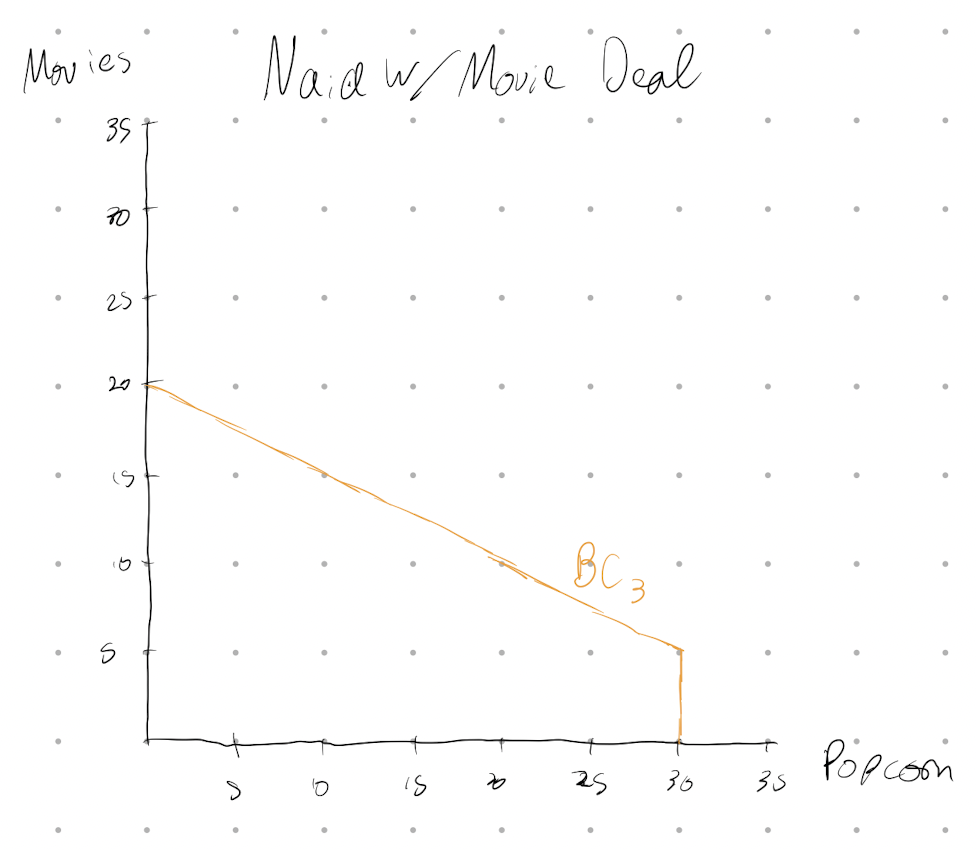
\includegraphics[width=10cm]{HW3Q6C}
\end{center}
\subsection*{Part D}
The movie theater will charge \$10 for the first 10 popcorns and \$2.5 for popcorns after the 10th popcorn.
\section{Non-Standard Budget Constraints}
\begin{center}
	\begin{tabular}{c|c}
		Muggle Magic Tricks (4) & Skiving Snackboxes (2, BOGO for first two snackboxes)\\
		\hline
		0 & 8 \\
		0.5 & 7\\
		1 & 6 \\
		2 & 4 \\
		2.5 & 2 \\
		3 & 0
	\end{tabular}
\end{center}
\begin{center}
	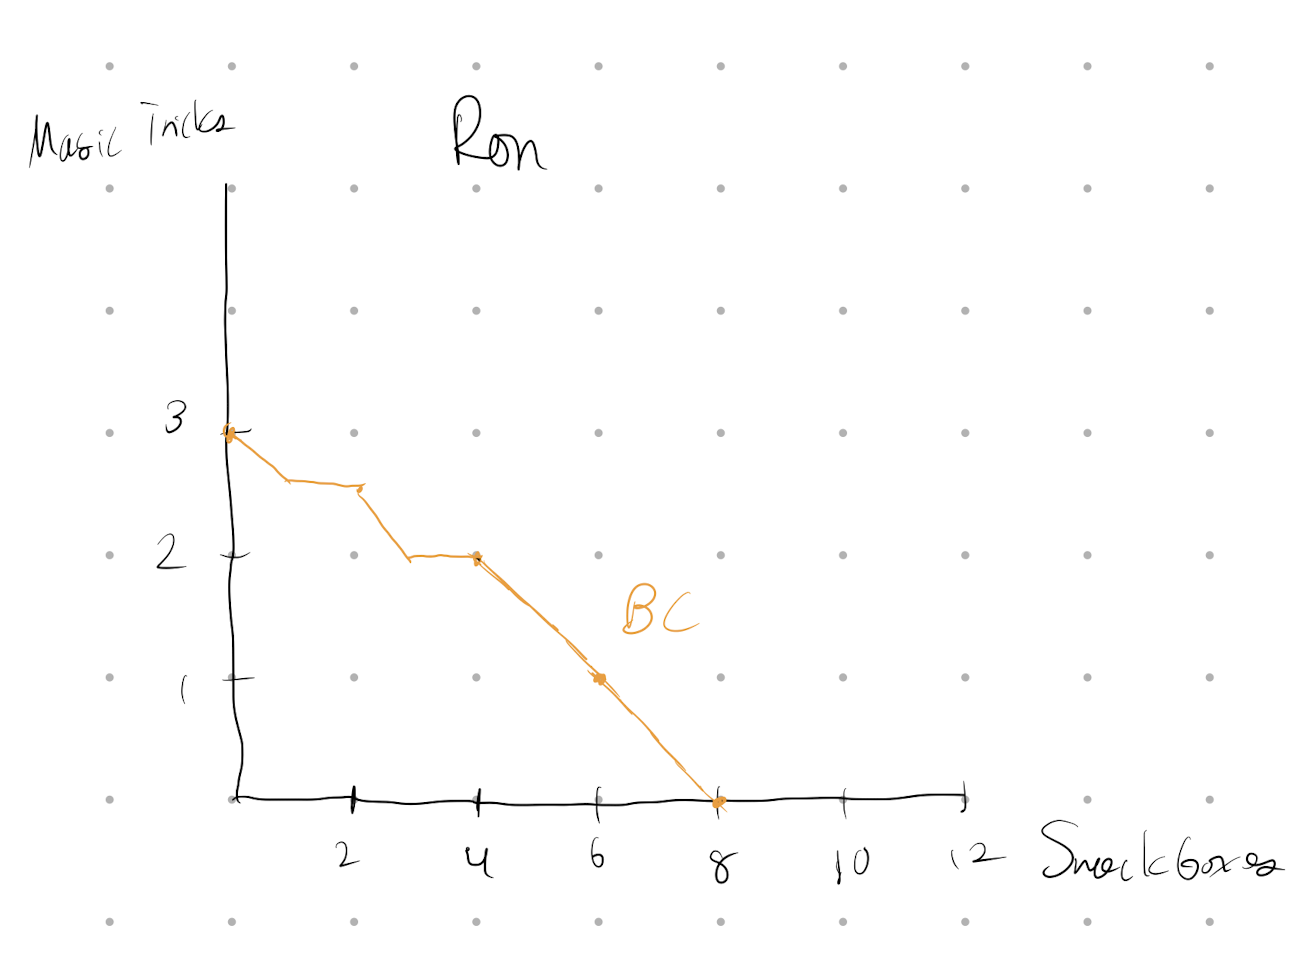
\includegraphics[width=10cm]{HW3Q7}
\end{center}
\section{Non-Standard Budget Constraints, cont'd}
\begin{center}
	\begin{tabular} {c|c}
		Ordinal Latte & Price \\
		\hline
		Latte 1 & \$4\\
		Latte 2 & \$12 \\
		Latte 3 & \$0 \\
		Latte 4 & \$2 \\
		Latte 5 & \$2
	\end{tabular}
\end{center}
\section{Utility Maximization}
The bundle we are aiming for is $5$ Cubanos and $25$ cheesesteaks, representing a $P_C$ of 6.4 in the budget constraint, which means the slope of the budget constraint is $\frac{5}{6.4} = 0.78$, which is not equal to the marginal rate of substitution of the utility function. Therefore, a bundle of $5$ cubanos and $25$ cheesesteaks is not optimal.
\section{Utility Maximization, cont'd}
\begin{align*}
	MRS_{WA} &= \frac{\frac{\partial U}{\partial W}}{\frac{\partial U}{\partial A}}\\
	&= \frac{3W^2A}{W^3} \\
	&= \frac{3A}{W} \\
	\frac{P_W}{P_A} &= \frac{1}{2} \\
	\frac{3A}{W} &= \frac{1}{2} \\
	W &= 6A \\
	6A + 3W &= 24 \\
	6A + 18A &= 24 \\
	A &= 1 \\
	W &= 6
\end{align*}
Phally will be \textbf{indifferent} to the deal offered because her optimal bundle of $6$ watercolors and $1$ acrylic paint will be unaffected by the proposed deal.
\begin{center}
	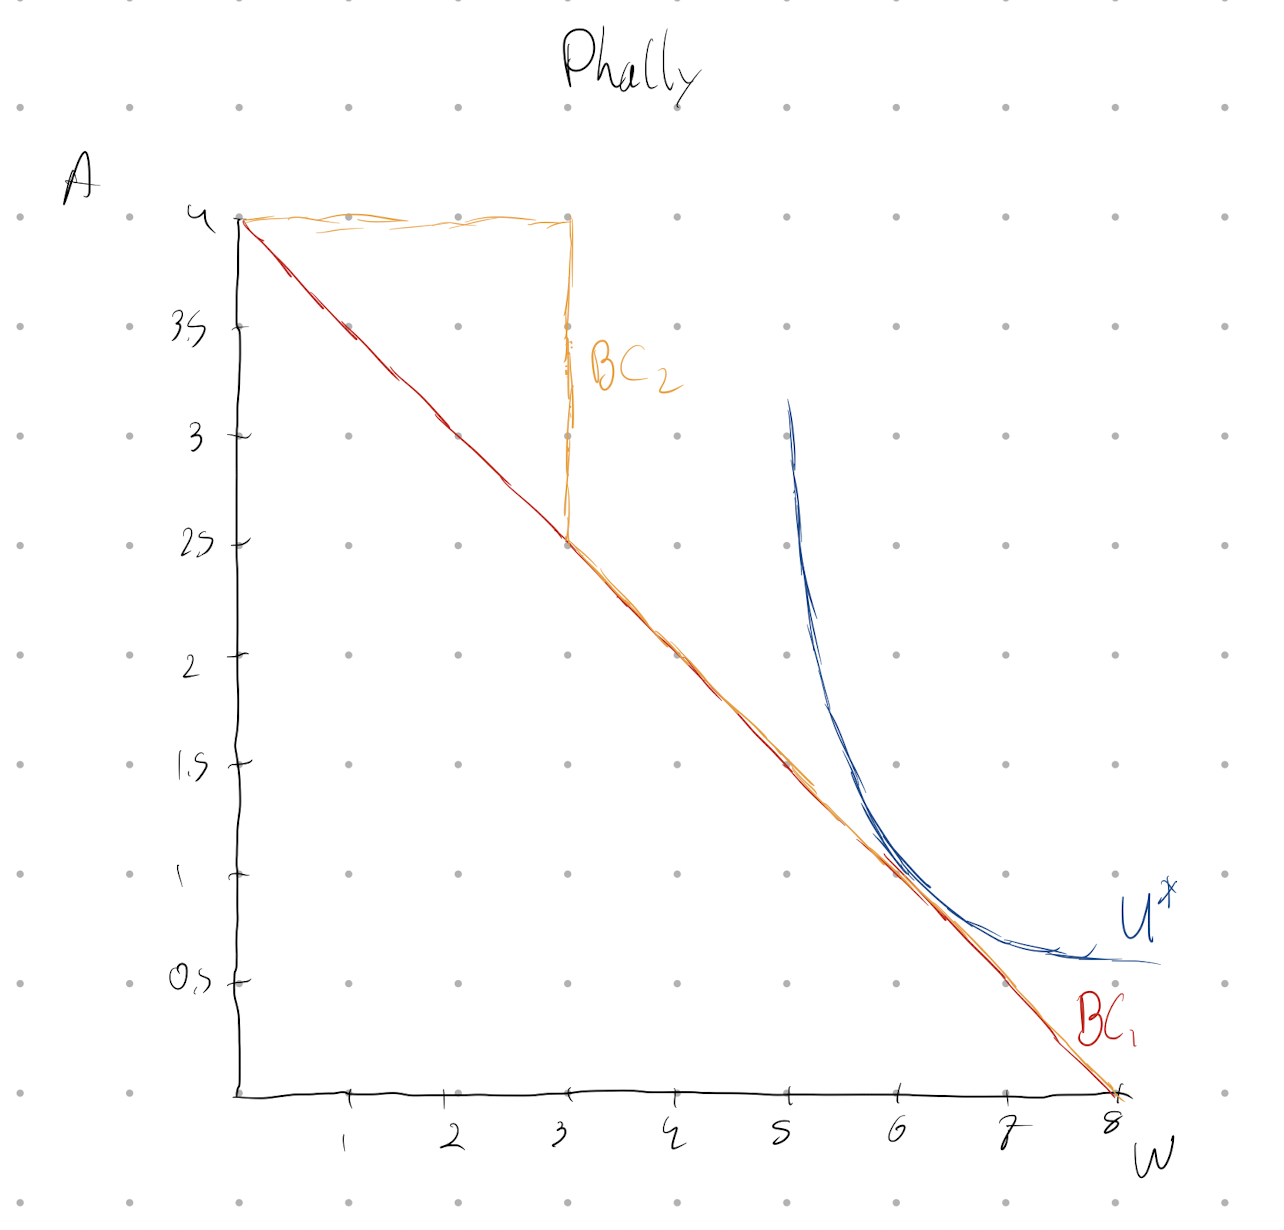
\includegraphics[width=10cm]{HW3Q10}
\end{center}
\section{Corner Solutions}
Yes, it is possible that Vanessa's optimal choice stays the same since the utility function might still be steeper than the new budget constraint curve.
\begin{center}
	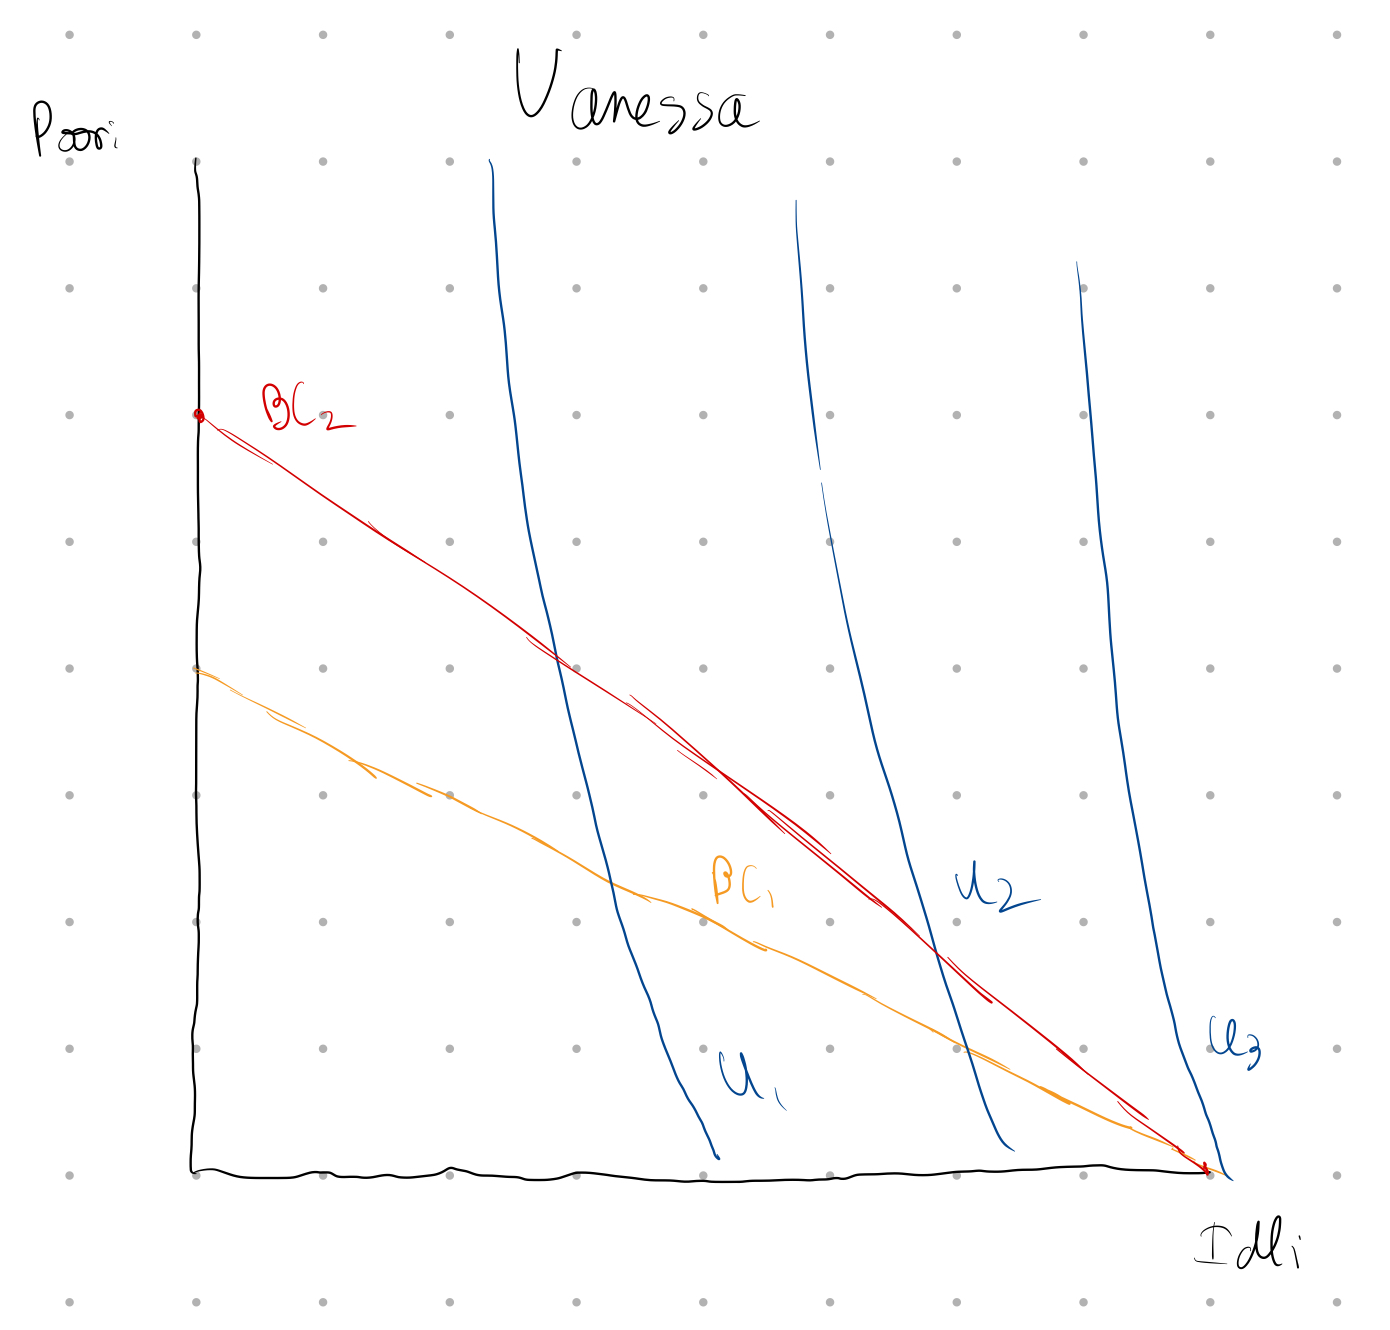
\includegraphics[width=10cm]{HW3Q11}
\end{center}
\section{Utility Maximization, Moving Decisions}
Gator will not move, as her optimal $ U' $ is less than her optimal $U$ at the current location, while Loki will move as his optimal $U'$ is greater than his optimal $U$ at his current location.
\begin{center}
	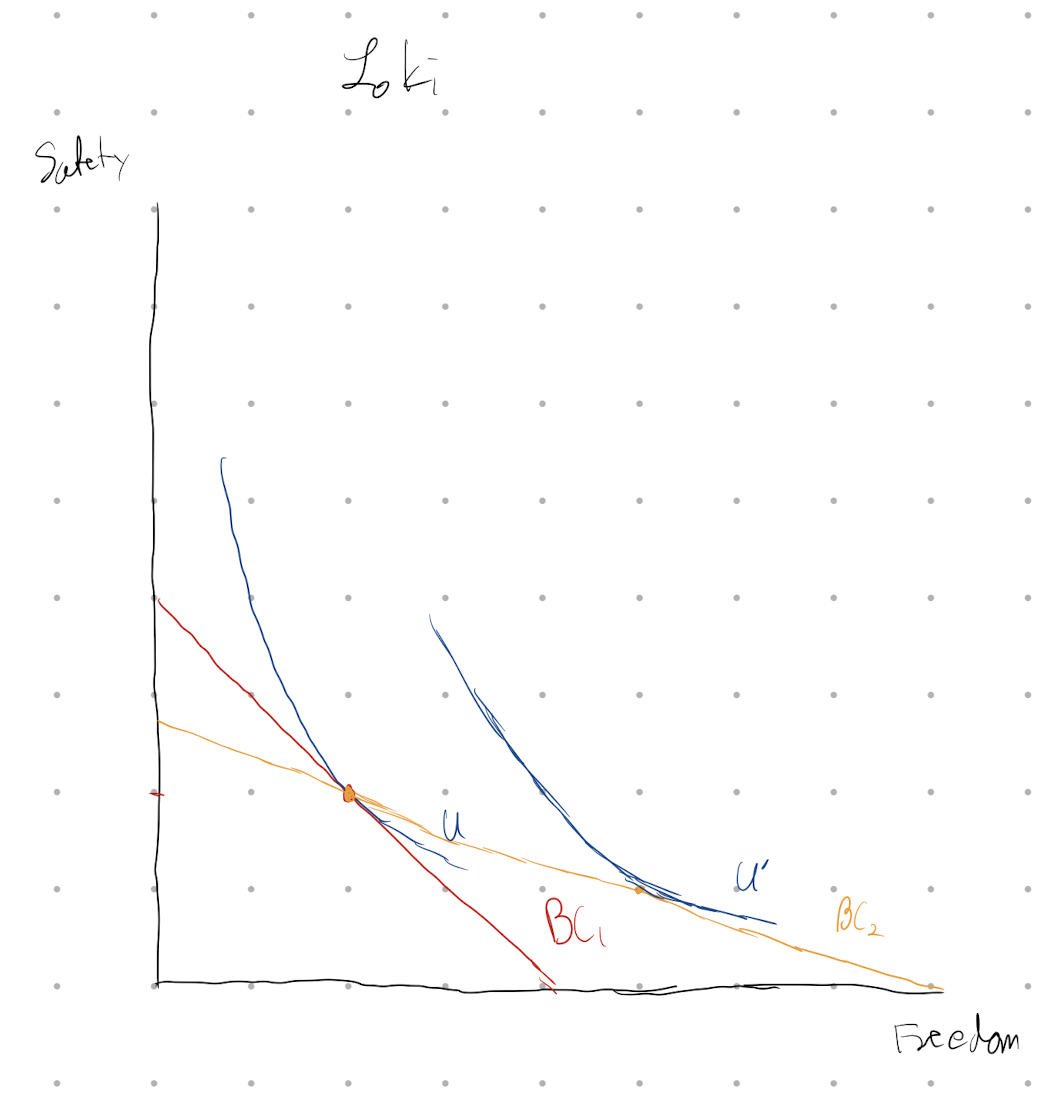
\includegraphics[width=10cm]{HW3Q12A}
	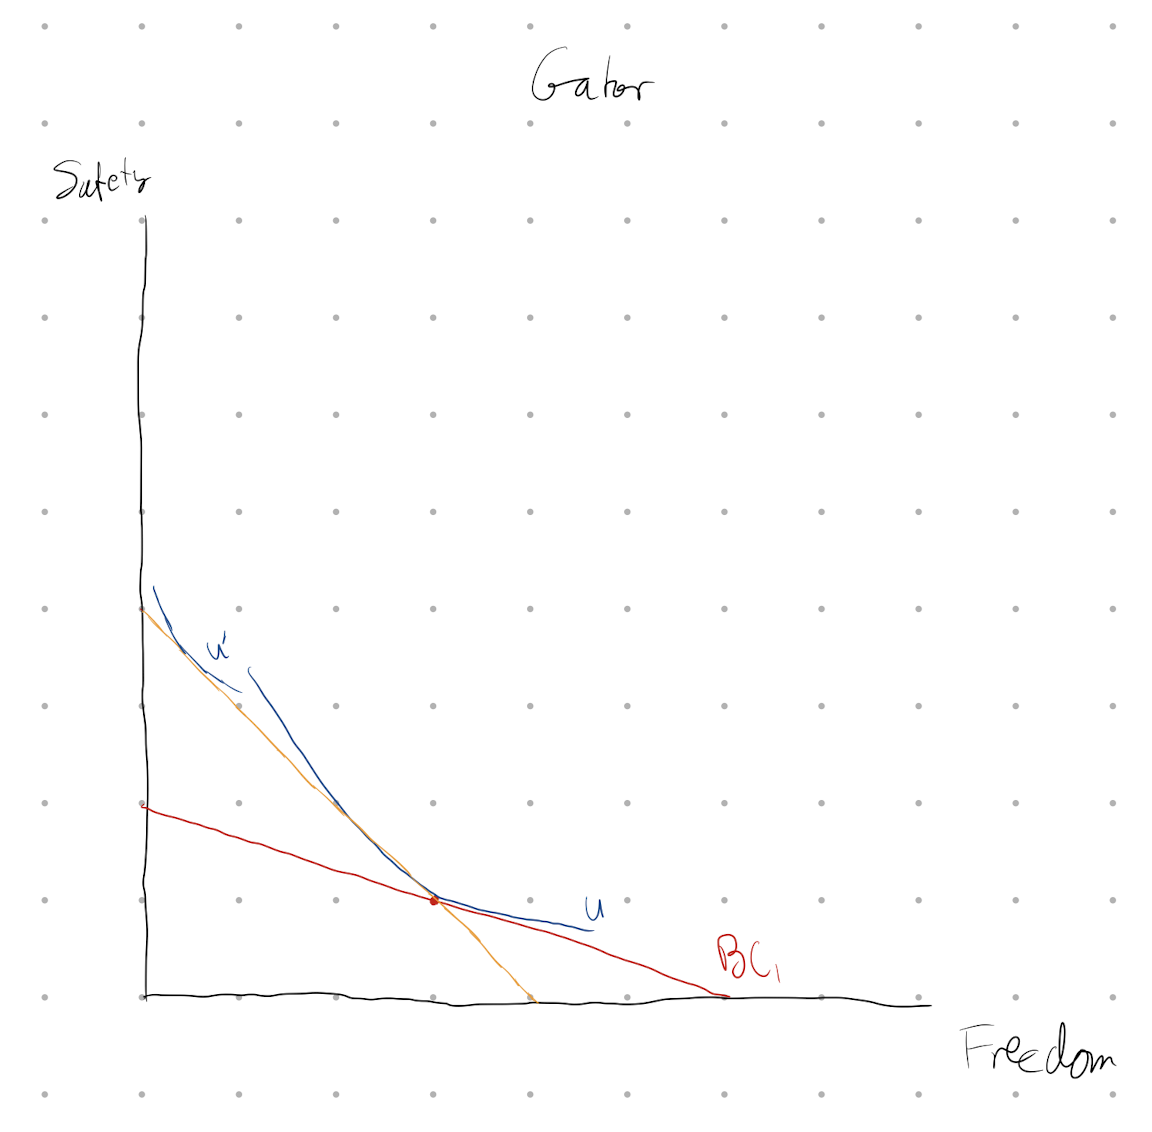
\includegraphics[width=10cm]{HW3Q12B}
\end{center}
}\end{document}
